\chapter{Future works}

While working on this thesis a few questions popped up in my brain :
\paragraph{Shortest reconfiguration path in the sliding token reconfiguration problem.}
\begin{flushleft}
    Shortest Sliding Token [Yamada and Uehara 2016]\\
    \textbf{Instance: } A yes-instance $(G, I, J)$ of Sliding Token, where $I, J$ are independent sets of a graph $G$. \\
    \textbf{Question: } Find a shortest TS-sequence that transforms $I$ into $J$ (and vice versa) \\
\end{flushleft}

%-------------------------------------------- Init --------------------------------------------
\begin{figure}[H]
    \centering
    \begin{subfigure}[b]{0.4\textwidth}
        \begin{scaletikzpicturetowidth}{\textwidth}
            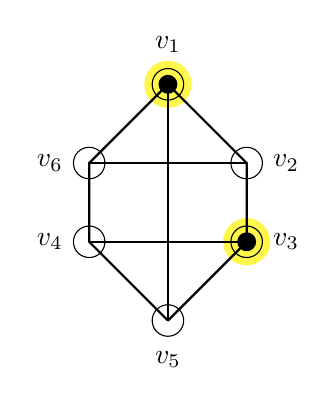
\begin{tikzpicture}[scale=1]
                \def\ver{0.12} %size of a vertex
                \def\xa{1}
                \def\ya{5}
                % highlight change
                \draw[fill=yellow, opacity=.7, draw=none] (\xa,\ya+3)  circle (0.3cm); % v1 ;
                \draw[fill=yellow, opacity=.7, draw=none] (\xa+1,\ya+1)  circle (0.3cm); % v3 ;

                %nodes
                \draw (\xa,\ya) circle (0.2cm);       % v5
                \draw (\xa+1,\ya+1) circle (0.2cm);   % v3
                \draw (\xa+1,\ya+2) circle (0.2cm);   % v2
                \draw (\xa,\ya+3) circle (0.2cm);     % v1
                \draw (\xa-1,\ya+2) circle (0.2cm);   % v6
                \draw (\xa-1,\ya+1) circle (0.2cm);   % v4

                %labels
                \node (1) at (\xa,\ya+3.5) {$v_1$};     % v1
                \node (2) at (\xa+1.5,\ya+2) {$v_2$};   % v2
                \node (3) at (\xa+1.5,\ya+1) {$v_3$};   % v3
                \node (5) at (\xa,\ya-0.5) {$v_5$};     % v5
                \node (4) at (\xa-1.5,\ya+1) {$v_4$};   % v4
                \node (6) at (\xa-1.5,\ya+2) {$v_6$};   % v6

                %token
                \path[fill] (\xa,\ya+3) circle (\ver);   % v1
                \path[fill] (\xa+1,\ya+1) circle (\ver);   % v3

                %edges
                \draw[thick] (\xa,\ya)--(\xa+1,\ya+1)--(\xa+1,\ya+2)--(\xa,\ya+3)--(\xa-1,\ya+2)--(\xa-1,\ya+1)--(\xa,\ya) ; % contour
                \draw[thick] (\xa,\ya)--(\xa,\ya+3) ;       % v5 - v1
                \draw[thick] (\xa+1,\ya+1)--(\xa-1,\ya+1) ; % v3 - v4
                \draw[thick] (\xa+1,\ya+2)--(\xa-1,\ya+2) ; % v2 - v6
            \end{tikzpicture}
        \end{scaletikzpicturetowidth}
        \caption{A $3$-regular graph $G=(V,E)$ and initial independent set $I_1 = \{v_1, v_3\}$}
        \label{fig:s1}
    \end{subfigure}
    \begin{subfigure}[b]{0.4\textwidth}
        \begin{scaletikzpicturetowidth}{\textwidth}
            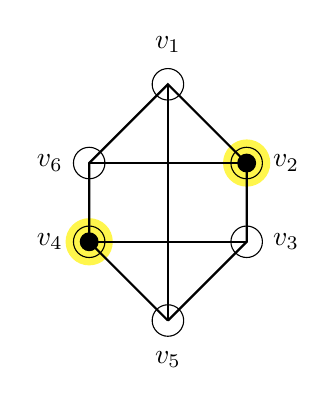
\begin{tikzpicture}[scale=1]
                \def\ver{0.12} %size of a vertex
                \def\xa{1}
                \def\ya{5}
                % highlight change
                \draw[fill=yellow, opacity=.7, draw=none] (\xa+1,\ya+2)  circle (0.3cm); % v2 ;
                \draw[fill=yellow, opacity=.7, draw=none] (\xa-1,\ya+1)  circle (0.3cm); % v4 ;

                %nodes
                \draw (\xa,\ya) circle (0.2cm);       % v5
                \draw (\xa+1,\ya+1) circle (0.2cm);   % v3
                \draw (\xa+1,\ya+2) circle (0.2cm);   % v2
                \draw (\xa,\ya+3) circle (0.2cm);     % v1
                \draw (\xa-1,\ya+2) circle (0.2cm);   % v6
                \draw (\xa-1,\ya+1) circle (0.2cm);   % v4

                %labels
                \node (1) at (\xa,\ya+3.5) {$v_1$};     % v1
                \node (2) at (\xa+1.5,\ya+2) {$v_2$};   % v2
                \node (3) at (\xa+1.5,\ya+1) {$v_3$};   % v3
                \node (5) at (\xa,\ya-0.5) {$v_5$};     % v5
                \node (4) at (\xa-1.5,\ya+1) {$v_4$};   % v4
                \node (6) at (\xa-1.5,\ya+2) {$v_6$};   % v6

                %token
                \path[fill] (\xa+1,\ya+2) circle (\ver);   % v2
                \path[fill] (\xa-1,\ya+1) circle (\ver);   % v4

                %edges
                \draw[thick] (\xa,\ya)--(\xa+1,\ya+1)--(\xa+1,\ya+2)--(\xa,\ya+3)--(\xa-1,\ya+2)--(\xa-1,\ya+1)--(\xa,\ya) ; % contour
                \draw[thick] (\xa,\ya)--(\xa,\ya+3) ;       % v5 - v1
                \draw[thick] (\xa+1,\ya+1)--(\xa-1,\ya+1) ; % v3 - v4
                \draw[thick] (\xa+1,\ya+2)--(\xa-1,\ya+2) ; % v2 - v6
            \end{tikzpicture}
        \end{scaletikzpicturetowidth}
        \caption{A $3$-regular graph $G=(V,E)$ and initial independent set $I_1 = \{v_1, v_3\}$}
        \label{fig:s2}
    \end{subfigure}
    \caption{Configuration-to-edge input instance}
    \label{fig:s1}
\end{figure}

%-------------------------------------------- shortest 1 --------------------------------------------
\begin{figure}[H]
    \centering
    \begin{subfigure}[b]{0.4\textwidth}
        \begin{scaletikzpicturetowidth}{\textwidth}
            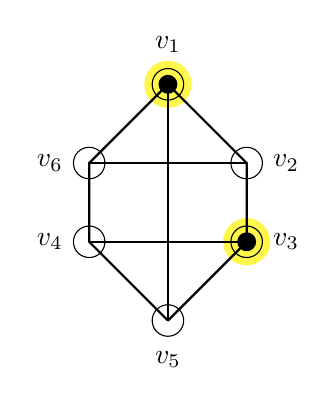
\begin{tikzpicture}[scale=1]
                \def\ver{0.12} %size of a vertex
                \def\xa{1}
                \def\ya{5}
                % highlight change
                \draw[fill=yellow, opacity=.7, draw=none] (\xa,\ya+3)  circle (0.3cm); % v1 ;
                \draw[fill=yellow, opacity=.7, draw=none] (\xa+1,\ya+1)  circle (0.3cm); % v3 ;

                %nodes
                \draw (\xa,\ya) circle (0.2cm);       % v5
                \draw (\xa+1,\ya+1) circle (0.2cm);   % v3
                \draw (\xa+1,\ya+2) circle (0.2cm);   % v2
                \draw (\xa,\ya+3) circle (0.2cm);     % v1
                \draw (\xa-1,\ya+2) circle (0.2cm);   % v6
                \draw (\xa-1,\ya+1) circle (0.2cm);   % v4

                %labels
                \node (1) at (\xa,\ya+3.5) {$v_1$};     % v1
                \node (2) at (\xa+1.5,\ya+2) {$v_2$};   % v2
                \node (3) at (\xa+1.5,\ya+1) {$v_3$};   % v3
                \node (5) at (\xa,\ya-0.5) {$v_5$};     % v5
                \node (4) at (\xa-1.5,\ya+1) {$v_4$};   % v4
                \node (6) at (\xa-1.5,\ya+2) {$v_6$};   % v6

                %token
                \path[fill] (\xa,\ya+3) circle (\ver);   % v1
                \path[fill] (\xa+1,\ya+1) circle (\ver);   % v3

                %edges
                \draw[thick] (\xa,\ya)--(\xa+1,\ya+1)--(\xa+1,\ya+2)--(\xa,\ya+3)--(\xa-1,\ya+2)--(\xa-1,\ya+1)--(\xa,\ya) ; % contour
                \draw[thick] (\xa,\ya)--(\xa,\ya+3) ;       % v5 - v1
                \draw[thick] (\xa+1,\ya+1)--(\xa-1,\ya+1) ; % v3 - v4
                \draw[thick] (\xa+1,\ya+2)--(\xa-1,\ya+2) ; % v2 - v6
            \end{tikzpicture}
        \end{scaletikzpicturetowidth}
        \caption{A $3$-regular graph $G=(V,E)$ and initial independent set $I_1 = \{v_1, v_3\}$}
        \label{fig:s11}
    \end{subfigure}
    \begin{subfigure}[b]{0.4\textwidth}
        \begin{scaletikzpicturetowidth}{\textwidth}
            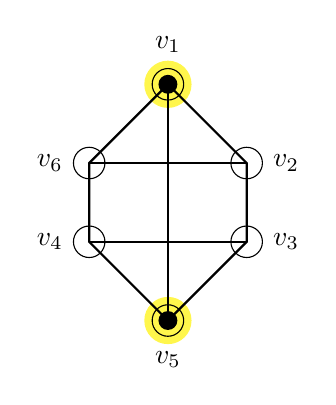
\begin{tikzpicture}[scale=1]
                \def\ver{0.12} %size of a vertex
                \def\xa{1}
                \def\ya{5}
                % highlight change
                \draw[fill=yellow, opacity=.7, draw=none] (\xa,\ya+3)  circle (0.3cm); % v1 ;
                \draw[fill=yellow, opacity=.7, draw=none] (\xa,\ya)  circle (0.3cm); % v5 ;

                %nodes
                \draw (\xa,\ya) circle (0.2cm);       % v5
                \draw (\xa+1,\ya+1) circle (0.2cm);   % v3
                \draw (\xa+1,\ya+2) circle (0.2cm);   % v2
                \draw (\xa,\ya+3) circle (0.2cm);     % v1
                \draw (\xa-1,\ya+2) circle (0.2cm);   % v6
                \draw (\xa-1,\ya+1) circle (0.2cm);   % v4

                %labels
                \node (1) at (\xa,\ya+3.5) {$v_1$};     % v1
                \node (2) at (\xa+1.5,\ya+2) {$v_2$};   % v2
                \node (3) at (\xa+1.5,\ya+1) {$v_3$};   % v3
                \node (5) at (\xa,\ya-0.5) {$v_5$};     % v5
                \node (4) at (\xa-1.5,\ya+1) {$v_4$};   % v4
                \node (6) at (\xa-1.5,\ya+2) {$v_6$};   % v6

                %token
                \path[fill] (\xa,\ya+3) circle (\ver);   % v1
                \path[fill] (\xa,\ya) circle (\ver);     % v5

                %edges
                \draw[thick] (\xa,\ya)--(\xa+1,\ya+1)--(\xa+1,\ya+2)--(\xa,\ya+3)--(\xa-1,\ya+2)--(\xa-1,\ya+1)--(\xa,\ya) ; % contour
                \draw[thick] (\xa,\ya)--(\xa,\ya+3) ;       % v5 - v1
                \draw[thick] (\xa+1,\ya+1)--(\xa-1,\ya+1) ; % v3 - v4
                \draw[thick] (\xa+1,\ya+2)--(\xa-1,\ya+2) ; % v2 - v6
            \end{tikzpicture}
        \end{scaletikzpicturetowidth}
        \caption{A $3$-regular graph $G=(V,E)$ and initial independent set $I_1 = \{v_1, v_3\}$}
        \label{fig:s12}
    \end{subfigure}
    \begin{subfigure}[b]{0.4\textwidth}
        \begin{scaletikzpicturetowidth}{\textwidth}
            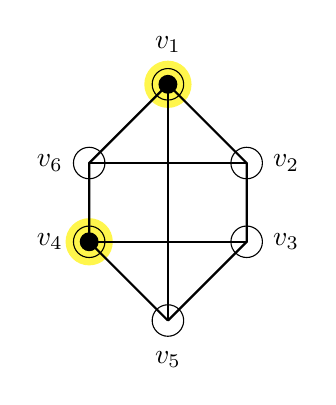
\begin{tikzpicture}[scale=1]
                \def\ver{0.12} %size of a vertex
                \def\xa{1}
                \def\ya{5}
                % highlight change
                \draw[fill=yellow, opacity=.7, draw=none] (\xa,\ya+3)  circle (0.3cm); % v1 ;
                \draw[fill=yellow, opacity=.7, draw=none] (\xa-1,\ya+1) circle (0.3cm); % v4 ;

                %nodes
                \draw (\xa,\ya) circle (0.2cm);       % v5
                \draw (\xa+1,\ya+1) circle (0.2cm);   % v3
                \draw (\xa+1,\ya+2) circle (0.2cm);   % v2
                \draw (\xa,\ya+3) circle (0.2cm);     % v1
                \draw (\xa-1,\ya+2) circle (0.2cm);   % v6
                \draw (\xa-1,\ya+1) circle (0.2cm);   % v4

                %labels
                \node (1) at (\xa,\ya+3.5) {$v_1$};     % v1
                \node (2) at (\xa+1.5,\ya+2) {$v_2$};   % v2
                \node (3) at (\xa+1.5,\ya+1) {$v_3$};   % v3
                \node (5) at (\xa,\ya-0.5) {$v_5$};     % v5
                \node (4) at (\xa-1.5,\ya+1) {$v_4$};   % v4
                \node (6) at (\xa-1.5,\ya+2) {$v_6$};   % v6

                %token
                \path[fill] (\xa,\ya+3) circle (\ver);   % v1
                \path[fill] (\xa-1,\ya+1) circle (\ver); % v4

                %edges
                \draw[thick] (\xa,\ya)--(\xa+1,\ya+1)--(\xa+1,\ya+2)--(\xa,\ya+3)--(\xa-1,\ya+2)--(\xa-1,\ya+1)--(\xa,\ya) ; % contour
                \draw[thick] (\xa,\ya)--(\xa,\ya+3) ;       % v5 - v1
                \draw[thick] (\xa+1,\ya+1)--(\xa-1,\ya+1) ; % v3 - v4
                \draw[thick] (\xa+1,\ya+2)--(\xa-1,\ya+2) ; % v2 - v6
            \end{tikzpicture}
        \end{scaletikzpicturetowidth}
        \caption{A $3$-regular graph $G=(V,E)$ and initial independent set $I_1 = \{v_1, v_3\}$}
        \label{fig:s13}
    \end{subfigure}
    \begin{subfigure}[b]{0.4\textwidth}
        \begin{scaletikzpicturetowidth}{\textwidth}
            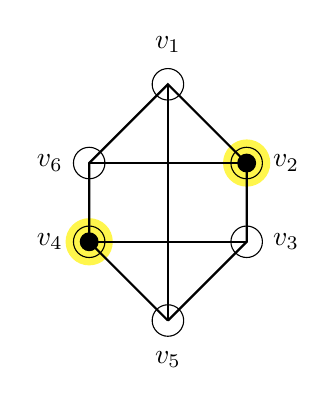
\begin{tikzpicture}[scale=1]
                \def\ver{0.12} %size of a vertex
                \def\xa{1}
                \def\ya{5}
                % highlight change
                \draw[fill=yellow, opacity=.7, draw=none] (\xa+1,\ya+2) circle (0.3cm); % v2 ;
                \draw[fill=yellow, opacity=.7, draw=none] (\xa-1,\ya+1) circle (0.3cm); % v4 ;

                %nodes
                \draw (\xa,\ya) circle (0.2cm);       % v5
                \draw (\xa+1,\ya+1) circle (0.2cm);   % v3
                \draw (\xa+1,\ya+2) circle (0.2cm);   % v2
                \draw (\xa,\ya+3) circle (0.2cm);     % v1
                \draw (\xa-1,\ya+2) circle (0.2cm);   % v6
                \draw (\xa-1,\ya+1) circle (0.2cm);   % v4

                %labels
                \node (1) at (\xa,\ya+3.5) {$v_1$};     % v1
                \node (2) at (\xa+1.5,\ya+2) {$v_2$};   % v2
                \node (3) at (\xa+1.5,\ya+1) {$v_3$};   % v3
                \node (5) at (\xa,\ya-0.5) {$v_5$};     % v5
                \node (4) at (\xa-1.5,\ya+1) {$v_4$};   % v4
                \node (6) at (\xa-1.5,\ya+2) {$v_6$};   % v6

                %token
                \path[fill] (\xa+1,\ya+2) circle (\ver); % v2
                \path[fill] (\xa-1,\ya+1) circle (\ver); % v4

                %edges
                \draw[thick] (\xa,\ya)--(\xa+1,\ya+1)--(\xa+1,\ya+2)--(\xa,\ya+3)--(\xa-1,\ya+2)--(\xa-1,\ya+1)--(\xa,\ya) ; % contour
                \draw[thick] (\xa,\ya)--(\xa,\ya+3) ;       % v5 - v1
                \draw[thick] (\xa+1,\ya+1)--(\xa-1,\ya+1) ; % v3 - v4
                \draw[thick] (\xa+1,\ya+2)--(\xa-1,\ya+2) ; % v2 - v6
            \end{tikzpicture}
        \end{scaletikzpicturetowidth}
        \caption{A $3$-regular graph $G=(V,E)$ and initial independent set $I_1 = \{v_1, v_3\}$}
        \label{fig:s13}
    \end{subfigure}
    \caption{Configuration-to-edge input instance}
    \label{fig:s2}
\end{figure}

%-------------------------------------------- shortest 2 --------------------------------------------
\begin{figure}[H]
    \centering
    \begin{subfigure}[b]{0.4\textwidth}
        \begin{scaletikzpicturetowidth}{\textwidth}
            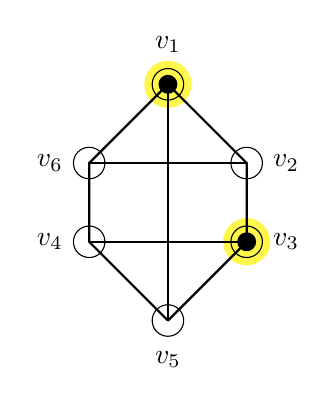
\begin{tikzpicture}[scale=1]
                \def\ver{0.12} %size of a vertex
                \def\xa{1}
                \def\ya{5}
                % highlight change
                \draw[fill=yellow, opacity=.7, draw=none] (\xa,\ya+3)  circle (0.3cm); % v1 ;
                \draw[fill=yellow, opacity=.7, draw=none] (\xa+1,\ya+1)  circle (0.3cm); % v3 ;

                %nodes
                \draw (\xa,\ya) circle (0.2cm);       % v5
                \draw (\xa+1,\ya+1) circle (0.2cm);   % v3
                \draw (\xa+1,\ya+2) circle (0.2cm);   % v2
                \draw (\xa,\ya+3) circle (0.2cm);     % v1
                \draw (\xa-1,\ya+2) circle (0.2cm);   % v6
                \draw (\xa-1,\ya+1) circle (0.2cm);   % v4

                %labels
                \node (1) at (\xa,\ya+3.5) {$v_1$};     % v1
                \node (2) at (\xa+1.5,\ya+2) {$v_2$};   % v2
                \node (3) at (\xa+1.5,\ya+1) {$v_3$};   % v3
                \node (5) at (\xa,\ya-0.5) {$v_5$};     % v5
                \node (4) at (\xa-1.5,\ya+1) {$v_4$};   % v4
                \node (6) at (\xa-1.5,\ya+2) {$v_6$};   % v6

                %token
                \path[fill] (\xa,\ya+3) circle (\ver);   % v1
                \path[fill] (\xa+1,\ya+1) circle (\ver);   % v3

                %edges
                \draw[thick] (\xa,\ya)--(\xa+1,\ya+1)--(\xa+1,\ya+2)--(\xa,\ya+3)--(\xa-1,\ya+2)--(\xa-1,\ya+1)--(\xa,\ya) ; % contour
                \draw[thick] (\xa,\ya)--(\xa,\ya+3) ;       % v5 - v1
                \draw[thick] (\xa+1,\ya+1)--(\xa-1,\ya+1) ; % v3 - v4
                \draw[thick] (\xa+1,\ya+2)--(\xa-1,\ya+2) ; % v2 - v6
            \end{tikzpicture}
        \end{scaletikzpicturetowidth}
        \caption{A $3$-regular graph $G=(V,E)$ and initial independent set $I_1 = \{v_1, v_3\}$}
        \label{fig:s11}
    \end{subfigure}
    \begin{subfigure}[b]{0.4\textwidth}
        \begin{scaletikzpicturetowidth}{\textwidth}
            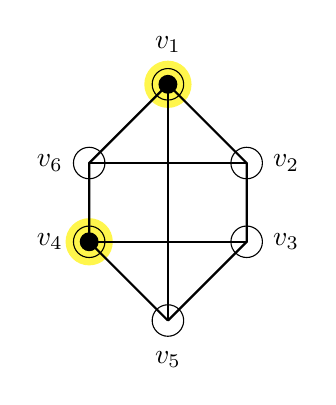
\begin{tikzpicture}[scale=1]
                \def\ver{0.12} %size of a vertex
                \def\xa{1}
                \def\ya{5}
                % highlight change
                \draw[fill=yellow, opacity=.7, draw=none] (\xa,\ya+3)  circle (0.3cm); % v1 ;
                \draw[fill=yellow, opacity=.7, draw=none] (\xa-1,\ya+1)  circle (0.3cm); % v4 ;

                %nodes
                \draw (\xa,\ya) circle (0.2cm);       % v5
                \draw (\xa+1,\ya+1) circle (0.2cm);   % v3
                \draw (\xa+1,\ya+2) circle (0.2cm);   % v2
                \draw (\xa,\ya+3) circle (0.2cm);     % v1
                \draw (\xa-1,\ya+2) circle (0.2cm);   % v6
                \draw (\xa-1,\ya+1) circle (0.2cm);   % v4

                %labels
                \node (1) at (\xa,\ya+3.5) {$v_1$};     % v1
                \node (2) at (\xa+1.5,\ya+2) {$v_2$};   % v2
                \node (3) at (\xa+1.5,\ya+1) {$v_3$};   % v3
                \node (5) at (\xa,\ya-0.5) {$v_5$};     % v5
                \node (4) at (\xa-1.5,\ya+1) {$v_4$};   % v4
                \node (6) at (\xa-1.5,\ya+2) {$v_6$};   % v6

                %token
                \path[fill] (\xa,\ya+3) circle (\ver);   % v1
                \path[fill] (\xa-1,\ya+1) circle (\ver); % v4

                %edges
                \draw[thick] (\xa,\ya)--(\xa+1,\ya+1)--(\xa+1,\ya+2)--(\xa,\ya+3)--(\xa-1,\ya+2)--(\xa-1,\ya+1)--(\xa,\ya) ; % contour
                \draw[thick] (\xa,\ya)--(\xa,\ya+3) ;       % v5 - v1
                \draw[thick] (\xa+1,\ya+1)--(\xa-1,\ya+1) ; % v3 - v4
                \draw[thick] (\xa+1,\ya+2)--(\xa-1,\ya+2) ; % v2 - v6
            \end{tikzpicture}
        \end{scaletikzpicturetowidth}
        \caption{A $3$-regular graph $G=(V,E)$ and initial independent set $I_1 = \{v_1, v_3\}$}
        \label{fig:s12}
    \end{subfigure}
    \begin{subfigure}[b]{0.4\textwidth}
        \begin{scaletikzpicturetowidth}{\textwidth}
            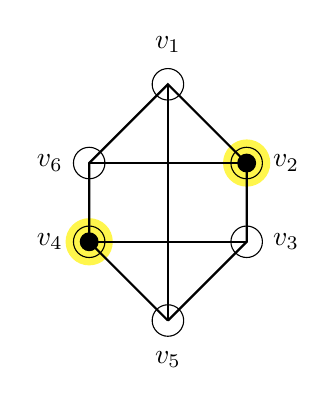
\begin{tikzpicture}[scale=1]
                \def\ver{0.12} %size of a vertex
                \def\xa{1}
                \def\ya{5}
                % highlight change
                \draw[fill=yellow, opacity=.7, draw=none] (\xa+1,\ya+2)  circle (0.3cm); % v2 ;
                \draw[fill=yellow, opacity=.7, draw=none] (\xa-1,\ya+1) circle (0.3cm); % v4 ;

                %nodes
                \draw (\xa,\ya) circle (0.2cm);       % v5
                \draw (\xa+1,\ya+1) circle (0.2cm);   % v3
                \draw (\xa+1,\ya+2) circle (0.2cm);   % v2
                \draw (\xa,\ya+3) circle (0.2cm);     % v1
                \draw (\xa-1,\ya+2) circle (0.2cm);   % v6
                \draw (\xa-1,\ya+1) circle (0.2cm);   % v4

                %labels
                \node (1) at (\xa,\ya+3.5) {$v_1$};     % v1
                \node (2) at (\xa+1.5,\ya+2) {$v_2$};   % v2
                \node (3) at (\xa+1.5,\ya+1) {$v_3$};   % v3
                \node (5) at (\xa,\ya-0.5) {$v_5$};     % v5
                \node (4) at (\xa-1.5,\ya+1) {$v_4$};   % v4
                \node (6) at (\xa-1.5,\ya+2) {$v_6$};   % v6

                %token
                \path[fill] (\xa+1,\ya+2) circle (\ver);   % v2
                \path[fill] (\xa-1,\ya+1) circle (\ver); % v4

                %edges
                \draw[thick] (\xa,\ya)--(\xa+1,\ya+1)--(\xa+1,\ya+2)--(\xa,\ya+3)--(\xa-1,\ya+2)--(\xa-1,\ya+1)--(\xa,\ya) ; % contour
                \draw[thick] (\xa,\ya)--(\xa,\ya+3) ;       % v5 - v1
                \draw[thick] (\xa+1,\ya+1)--(\xa-1,\ya+1) ; % v3 - v4
                \draw[thick] (\xa+1,\ya+2)--(\xa-1,\ya+2) ; % v2 - v6
            \end{tikzpicture}
        \end{scaletikzpicturetowidth}
        \caption{A $3$-regular graph $G=(V,E)$ and initial independent set $I_1 = \{v_1, v_3\}$}
        \label{fig:s13}
    \end{subfigure}
    \caption{Configuration-to-edge input instance}
    \label{fig:s2}
\end{figure}

\begin{theorem}(Kaminski et al. 2012)
It is $\NP$-complete to decide if there is a TS-sequence having at most $l$ token-slides between two independent sets $I, J$ of a
perfect graph $G$ even when $l$ is polynomial in $|V(G)|$.
\end{theorem}

\begin{theorem}(Kaminski et al. 2012)
Shortest Sliding Token can be solved in linear time for cographs (P4-free graphs).
\end{theorem}

\begin{theorem}(Yamada and Uehara 2016)
Shortest Sliding Token can be solved in polynomial time for proper interval graphs, trivially perfect graphs, and caterpillars.
\end{theorem}

\begin{theorem}(Sugimori, AAAC 2018)
Shortest Sliding Token can be solved in $O(poly(n))$ time when the input graph is a tree T on n vertices.
\end{theorem}

\begin{theorem}(Ryuhei Uehara, CIAC 2019)
Shortest Sliding Token can be solved in $O(n^2)$ time when the input graph is a spider G (i.e., a tree having exactly one
vertex of degree at least $3$) on $n$ vertices.
\end{theorem}


\paragraph{St-Conn(S) problem in NCL.}

\paragraph{Can schaefer's dichotomy be applied to the 3-move subset sum reconfiguration problem i.e can we have a tight result for $k \leq 3$ and $k \geq 3 ? $}

\paragraph{Finding an optimal $k < 23$ for the colour classes of the exact cover problem. More en rapport avec le path in hypercube.}
